% **************************************************
% Document Class Definition
% **************************************************
\documentclass[%
    paper=A4,               % paper size --> A4 is default in Germany
    twoside=true,           % onesite or twoside printing
    openright,              % doublepage cleaning ends up right side
    parskip=full,           % spacing value / method for paragraphs
    chapterprefix=true,     % prefix for chapter marks
    11pt,                   % font size
    headings=normal,        % size of headings
    bibliography=totoc,     % include bib in toc
    listof=totoc,           % include listof entries in toc
    titlepage=on,           % own page for each title page
    captions=tableabove,    % display table captions above the float env
    draft=false,            % value for draft version
]{scrreprt}%


% **************************************************
% Setup YOUR thesis document in this file !
% **************************************************
% !TEX root = main.tex


% **************************************************
% Files' Character Encoding
% **************************************************
\PassOptionsToPackage{utf8}{inputenc}
\usepackage{inputenc}


% **************************************************
% Information and Commands for Reuse
% **************************************************
\newcommand{\thesisTitle}{Ranking of Classification Algorithms in AutoML}
\newcommand{\thesisName}{Helena Graf}
\newcommand{\thesisSubject}{Bachelor’s Thesis}
\newcommand{\thesisDate}{January 5, 2018}
\newcommand{\thesisVersion}{My First Draft}

\newcommand{\thesisFirstReviewer}{Prof. Dr. Eyke Hüllermeier}
\newcommand{\thesisFirstReviewerUniversity}{\protect{Paderborn University}}
\newcommand{\thesisFirstReviewerDepartment}{Department of Computer Science}

\newcommand{\thesisSecondReviewer}{Prof. Dr. Axel-Cyrille Ngonga-Ngomo}
\newcommand{\thesisSecondReviewerUniversity}{\protect{Paderborn University}}
\newcommand{\thesisSecondReviewerDepartment}{Department of Computer Science}

\newcommand{\thesisFirstSupervisor}{Prof. Dr. Eyke Hüllermeier}
\newcommand{\thesisSecondSupervisor}{Prof. Dr. Axel-Cyrille Ngonga-Ngomo}

\newcommand{\thesisUniversity}{Paderborn University}
\newcommand{\thesisUniversityDepartment}{Department of Computer Science}
\newcommand{\thesisUniversityInstitute}{}
\newcommand{\thesisUniversityGroup}{Intelligent Systems Group (ISG)}
\newcommand{\thesisUniversityCity}{Paderborn}
\newcommand{\thesisUniversityStreetAddress}{Pohlweg 51}
\newcommand{\thesisUniversityPostalCode}{33098}

% **************************************************
% Debug LaTeX Information
% **************************************************
%\listfiles


% **************************************************
% Load and Configure Packages
% **************************************************
\usepackage[english]{babel} % babel system, adjust the language of the content
\PassOptionsToPackage{% setup clean thesis style
    figuresep=colon,%
    sansserif=false,%
    hangfigurecaption=false,%
    hangsection=true,%
    hangsubsection=true,%
    colorize=full,%
    colortheme=upbisg,%
    bibsys=biber,%
    bibfile=bib-refs,%
    bibstyle=alphabetic,%
    wrapfooter=false,%
}{cleanthesis}
\usepackage{cleanthesis}

\usepackage{mathtools}
\usepackage{amsmath}
\usepackage{amssymb}
\usepackage{amsthm}
\theoremstyle{definition}
\usepackage{tikz}
\usepackage{xcolor}

% Colour Definitions
\definecolor{uniblue}{RGB}{000,032,091}
\definecolor{unigrey}{RGB}{199,201,199}
\definecolor{uniaccentblue}{RGB}{000,163,224}

\hypersetup{% setup the hyperref-package options
    pdftitle={\thesisTitle},    %   - title (PDF meta)
    pdfsubject={\thesisSubject},%   - subject (PDF meta)
    pdfauthor={\thesisName},    %   - author (PDF meta)
    plainpages=false,           %   -
    colorlinks=false,           %   - colorize links?
    pdfborder={0 0 0},          %   -
    breaklinks=true,            %   - allow line break inside links
    bookmarksnumbered=true,     %
    bookmarksopen=true          %
}



% **************************************************
% Document CONTENT
% **************************************************
\begin{document}

% --------------------------
% rename document parts
% --------------------------
%\renewcaptionname{ngerman}{\figurename}{Abb.}
%\renewcaptionname{ngerman}{\tablename}{Tab.}
\renewcaptionname{english}{\figurename}{Fig.}
\renewcaptionname{english}{\tablename}{Tab.}
\newtheorem{defn}{Definition}
% --------------------------
% Front matter
% --------------------------
\pagenumbering{roman}			% roman page numbing (invisible for empty page style)
\pagestyle{empty}				% no header or footers
% !TEX root = ../main.tex
%
% ------------------------------------  --> cover title page
\begin{titlepage}
	\pdfbookmark[0]{Cover}{Cover}
	\flushright
	\hfill
	\vfill
	{\LARGE\thesisTitle \par}
	\rule[5pt]{\textwidth}{.4pt} \par
	{\Large\thesisName}
	\vfill
	\textit{\large\thesisDate} \\
	Version: \thesisVersion
\end{titlepage}


% ------------------------------------  --> main title page
\begin{titlepage}
	\pdfbookmark[0]{Titlepage}{Titlepage}
	\tgherosfont
	
	\begin{figure}
	\begin{minipage}[t]{8.5cm}		
	
\includegraphics[height=1.8cm]{gfx/upb_1E}\\
	\textsf{\small{\hspace*{1.3cm}Department of Electrical Engineering,\\
	\hspace*{1.3cm}Computer Science and Mathematics\\
%		\hspace*{1.3cm}Institute of Computer Science\\
		\hspace*{1.3cm}Warburger Straße 100 \\
		\hspace*{1.3cm}33098 Paderborn
		}}
	\end{minipage}
	\hfill
	\begin{minipage}[t]{4.7cm}
	
\includegraphics[height=1.8cm]{gfx/is-logo-klein}\\
	\textsf{%Institute of Computer Science\\
	\hspace*{0.1cm}\small{Intelligent Systems Group (ISG)}
	}
	\end{minipage}
	\end{figure}
	
	\centering
	%\textsf{\thesisUniversityDepartment} \\
	%\textsf{\thesisUniversityInstitute} \\
	%\textsf{\thesisUniversityGroup} \\

	\vfill
	{\large \thesisSubject} \\[5mm]
	{\LARGE \color{ctcolortitle}\textbf{\thesisTitle} \\[10mm]}
	{\Large \thesisName} \\[5mm]
	{Matriculation Number: 7011643}\\

	\vfill
	\begin{minipage}[t]{.27\textwidth}
		\raggedleft
		\textit{1. Reviewer}
	\end{minipage}
	\hspace*{15pt}
	\begin{minipage}[t]{.65\textwidth}
		{\Large \thesisFirstReviewer} \\
	  	{\small \thesisFirstReviewerDepartment} \\[-1mm]
		{\small \thesisFirstReviewerUniversity}
	\end{minipage} \\[5mm]
	\begin{minipage}[t]{.27\textwidth}
		\raggedleft
		\textit{2. Reviewer}
	\end{minipage}
	\hspace*{15pt}
	\begin{minipage}[t]{.65\textwidth}
		{\Large \thesisSecondReviewer} \\
	  	{\small \thesisSecondReviewerDepartment} \\[-1mm]
		{\small \thesisSecondReviewerUniversity}
	\end{minipage} \\[10mm]
	\begin{minipage}[t]{.27\textwidth}
		\raggedleft
		\textit{Supervisors}
	\end{minipage}
	\hspace*{15pt}
	\begin{minipage}[t]{.65\textwidth}
		\thesisFirstSupervisor\ and \thesisSecondSupervisor
	\end{minipage} \\[10mm]

	\thesisDate \\

\end{titlepage}


% ------------------------------------  --> lower title back for single page layout
\hfill
\vfill
{
	\small
	\textbf{\thesisName} \\
	\textit{\thesisTitle} \\
	\thesisSubject, \thesisDate \\
	Reviewers: \thesisFirstReviewer\ and \thesisSecondReviewer \\
	Supervisors: \thesisFirstSupervisor\ and \thesisSecondSupervisor \\[1.5em]
	\textbf{\thesisUniversity} \\
	\textit{\thesisUniversityGroup} \\
	% No institute
	%\thesisUniversityInstitute \\
	\thesisUniversityDepartment \\
	\thesisUniversityStreetAddress \\
	\thesisUniversityPostalCode\ and \thesisUniversityCity
}
		% INCLUDE: all titlepages
\cleardoublepage

\pagestyle{plain}				% display just page numbers
% !TEX root = ../my-thesis.tex
%
\pdfbookmark[0]{Abstract}{Abstract}
\chapter*{Abstract}
\label{sec:abstract}
\vspace*{-10mm}

Should abstract be included?

\vspace*{20mm}

{\usekomafont{chapter}Abstract (different language)}\label{sec:abstract-diff} \\

Und falls ja, dann zweisprachig?
		% INCLUDE: the abstracts (english and german)
\cleardoublepage
%
% !TEX root = ../my-thesis.tex
%
\pdfbookmark[0]{Acknowledgement}{Acknowledgement}
\chapter*{Acknowledgement}
\label{sec:acknowledgement}
\vspace*{-10mm}

Including acknowledgement expected or frowned upon for undergrad thesis?
 % INCLUDE: acknowledgement
\cleardoublepage
%
\setcounter{tocdepth}{2}		% define depth of toc
\tableofcontents				% display table of contents
\cleardoublepage

% --------------------------
% Body matter
% --------------------------
\pagenumbering{arabic}			% arabic page numbering
\setcounter{page}{1}			% set page counter
\pagestyle{maincontentstyle} 	% fancy header and footer

% Move from general to specific
\chapter{Introduction}
\label{sec:intro}

%% Context
% Need more automated analysis of data
The potential of big data is evident, and an increasing amount of information is collected and available for analysis - but this potential is not utilized. In a white paper, the International Data Corporation claims that in 2012, out of the 2.8 zettabytes (ZB) of available data only 3\% were tagged as to enable further processing, and only 0.5\% were analyzed \cite{gantz2012the}. A follow-up paper in 2017 projects that in 2025, 15\% of the estimated 163ZB of global data will be tagged, and approximately 3\% analyzed \cite{gantz2017data}. While this is more optimistic, it still shows that there is a huge gap between the amount of data that could potentially be used and the amount of data actually available. This indicates that the demand of data to be analyzed cannot be covered by data scientists alone, and the process is not accessible enough to non-experts. It thus calls for automation of the process in a way that not much expertise in the field of machine learning is needed to gain insights about the collected data.

% Of ML, tasks, classification is important & classifier performances vary across data sets, so it is not easy to just pick one
One of the most prominent machine learning tasks is classification: A class is assigned to an instance, for example clients of a bank may be either deemed creditworthy or not, based on factors like other existing credits or the job of the client. But selecting a fitting classifier for a new data set is difficult, since algorithm performances can vary substantially among data sets, and it is not feasible to simply apply a large number of them to empirically find a good match. For example, on a data set about the electricity prices in the Australian state New South Wales \cite{harris1999splice}, the predictive accuracy for the Multilayer Perceptron\footnote{With standard hyperparameters (L:0.3,M:0.2,N:500,V:0,S:0,E:20,H:a).} is 0.7887 \cite{cachada2017run3}. The predictive accuracy of the Random Forest\footnote{With standart hyperparameters (P:100,I:100,num-slots:1,K:0,M:1.0,V:0.001,S:1).} algorithm on the same data set is 0.9236 \cite{cachada2017run}, a much higher value. On a different data set, with the topic of vehicle silhouettes \cite{siebert1987vehicle}, we get a predictive accuracy of 0.7979 for the Multilayer Perceptron \cite{cachada2017run4}, and 0.7518 for Random Forests \cite{cachada2017run2}, showing an advantage of the former on this data set\footnote{Hyperparameters as above.}. So in each case, one would have picked a different algorithm in order to achieve the best results, and this example just illustrates the choice between two algorithms - in reality, the number of available algorithms is much larger. In general, this means that for a different data set, a different algorithm might yield the best performance.

\section{Problem Statement}
\label{sec:intro:problem}
%% Problem + Significance
Since there is no one best classifier for all data sets, it can be concluded that how well a classifier performs on a given data set is dependent on certain properties of the data set. Combined with the need for automated machine learning and the importance but difficulty of selecting a fitting classification algorithm, this calls for an approach that properties of data sets to automatically suggest well-performing classifiers for a new problem.

%% Response
% Therefore the goal is testing the this assumption if possible by using regression algos and preference learning
Thus, the aim of this thesis is the implementation and evaluation of two different approaches to ranking classification algorithms based on past-performances of the algorithms and according to properties of the data set. The two approaches include one regression-based approach that breaks down the problem of predicting a ranking into predicting a single performance value for each algorithm and then ranking them accordingly, and a preference based approach that is concerned with learning the rankings directly. Especially in the case of regression based ranking there is reason to believe that such a prediction is possible, as regression models have been used successfully to predict the performance of an algorithm dependent on the hyperparameter configuration \cite{DBLP:conf/aaai/EggenspergerHHL15}.

\section{Thesis Structure}
\label{sec:intro:structure}
%% Roadmap
The following paragraphs give an outline of the thesis structure by providing a brief summary of each chapter.

\textbf{Chapter \ref{sec:fundamentals} - \nameref{sec:fundamentals}} \\[0.2em]
% Begin with fundamentals to give a brief overview of the field of ML relevant to this thesis
First, some preliminaries are discussed. A brief overview of tasks from the field of machine learning which are relevant to this thesis is given, and methods used for evaluation are explained. 

\textbf{Chapter \ref{sec:approach} - \nameref{sec:approach}} \\[0.2em]
% Continue with description of the approach to the problem described in detail
The next chapter continues by describing the approach of this thesis for ranking classification algorithms. The two different proposed methods are contrasted. Following the details of the approach, the implementation thereof is presented. Used software libraries are pointed out.

% How the conducted experiments have been set up and discussion of results
\textbf{Chapter \ref{sec:evaluation} - \nameref{sec:evaluation}} \\[0.2em]
The evaluation of the different ranking implementations is described by first clarifying the experimental setup used for the evaluation, followed by a discussion of the results.

% Visit more work
\textbf{Chapter \ref{sec:related} - \nameref{sec:related}} \\[0.2em]
After the approach of this thesis has been laid out in detail, the scope is extended to related work in the area of AutoML in general and ranking of learning algorithms more specifically. Differences and similarities in the approaches are discussed briefly.

\textbf{Chapter \ref{sec:conclusion} - \nameref{sec:conclusion}} \\[0.2em]
% Conlude + future work
In the last chapter, the results which have been achieved are revisited with the goals in mind, and future work is outlined.

   % INCLUDE: introduction
% !TEX root = ../my-thesis.tex
%
\chapter{Fundamentals}
\label{sec:fundamentals}

The core topic of this thesis falls under the category of machine learning. Thus, firstly the concept of machine learning and the   

\section{Machine Learning}
In this section, the aspects of the field of machine learning which are relevant for this thesis are going to be introduced briefly. The core of machine learning is learning algorithms, which are used to induce a general model from a set of data samples. The concept of machine learning will be explained here with the help of an example. % Further what happens exactly here 

Suppose an aspiring gardener wants to learn how to distinguish between different species of iris plants, a genus of ornamental plants with colorful flowers. More specifically, the focus lies on the three species iris versicolor, virginica and setosa. In order to do so, the gardener has observed four different \textit{features}, namely the length and width of their petals and sepals, for a number of different individuals for which he knows the species. The goal of the gardener is then to learn how to distinguish the species based on these features, that is to derive a \textit{model} from the data that will predict which species (out of the considered the three) an unknown iris plant is. The gardener decides to build a decision tree from the data with forks on the basis of feature values, so that they can determine the species of the plant without much calculation. They observe that all iris setosa plants from his sample have a petal width of $\leq 0.6 $ cm, and that of the plants with a petal width of $>0.6$ cm, most plants with a petal width $\leq 1.7$ cm are of the iris versicolor species. The remaining plants with a petal width of $>1.7$ cm are mostly iris virginica plants. While this model will not correctly predict the species of all iris plants, the gardener is settles with the approximation they have found.

\begin{table}[h]
	\begin{tabularx}{\textwidth}{>{\hsize=1.1\hsize}X >{\hsize=0.8\hsize\centering\arraybackslash}X >{\hsize=0.8\hsize\centering\arraybackslash}X >{\hsize=0.8\hsize\centering\arraybackslash}X >{\hsize=0.8\hsize\centering\arraybackslash}X  >{\hsize=1.7\hsize}X}
		%\hline
		Feature	& \multicolumn{1}{>{\hsize=0.8\hsize}X}{Sepal length}	& \multicolumn{1}{>{\hsize=0.8\hsize}X}{Sepal width}	& \multicolumn{1}{>{\hsize=0.8\hsize}X}{Petal length}	& \multicolumn{1}{>{\hsize=0.8\hsize}X}{Petal width} 	& Species			\\ \hline
				& 5.1			& 3.5			& 1.4			& 0.2			& Iris setosa		\\ 
				& 5.0			& 3.5			& 1.6			& 0.6			& Iris setosa		\\ 
				& 5.0			& 3.4			& 1.6			& 0.4			& Iris setosa		\\ 
				& 5.6			& 3.0			& 4.5			& 1.5			& Iris versicolor	\\ 				
				& 6.7			& 3.1			& 4.4			& 1.4			& Iris versicolor	\\ 	
				& 5.9			& 3.2			& 4.8			& 1.8			& Iris versicolor	\\ 	
				& 7.2			& 3.0			& 5.8			& 1.6			& Iris virginica		\\ 	
				& 5.9			& 3.0			& 5.1			& 1.8			& Iris virginica		\\ 
				& 6.9			& 3.1			& 5.1			& 2.3			& Iris virginica		\\ 	
	\end{tabularx}
	\label{tab:iris}
	\caption{Example values for the predictive accuracy of classifiers (data set not relevant in this context). The predictive accuracy denotes the percentage of instances for which the classifier correctly perdicted the class membership.}
\end{table}

In formal terms, the gardener is searching for an unknown \textit{target function} $f:X \rightarrow Y$ from the input space $X$ to the output space $Y$ that represents an ideal way of identifying iris species. $X$ denotes the possible inputs, in this case all combinations of the four features that have been defined, whereas $Y$ are the outputs, here the species of iris plant. The examples that the gardener recorded are samples $(x_1,y_1),\dots,(x_n,y_n)$ from $f$ such that $f(x_i)=y_i$. Together, they form a data set $D$ which is one of all possible data sets $\mathbb{D}$ for the problem. He then chooses a specific approximation $g:X \rightarrow Y,g\approx f$, the decision tree they built, from the hypothesis space $H$, which in this case consists of possible decision trees. The learning algorithm itself thus maps a data set to a hypothesis from the hypothesis space and can be defined as $A:\mathbb{D}\rightarrow H$.

%TODO include picture of the models etc + table + decision tree that is built

\subsection{Supervised Learning}
The problem described above has some additional properties besides being a machine learning problem in general. Firstly, it falls in the category of supervised machine learning. Supervised learning is one of the three main learning paradigms of machine learning, together with reinforcement learning and unsupervised learning. In the context of this thesis, the latter will be neglected as only supervised learning is used. It is characterized by the fact that the learning algorithm is provided with a set of inputs \textit{together} with the outputs, which could be viewed as a kind of teacher, or supervisor, explaining expected results to the learner. In the other cases, no such detailed feedback is provided to the learner. 

\subsection{Classification and Regression}
%TODO instance explained before here?
In addition to falling into the category of supervised learning, the problem is a classification problem. The nature of the prediction is to assign one of the three classes, or labels, 'iris setosa', iris virginica' and 'iris versicolor' to a new plant. Formally, this means that the output space $Y$ of the target function consist of a finite set of labels $\lbrace y_1,\dots,y_n\rbrace$, so that each instance is associated with a label $y_i \in Y$, in this case $Y=\lbrace 'iris-setosa','iris virginica', 'iris versicolor' \rbrace $. 

Apart from classification, another important category of machine learning problems is regression problems. In the case of regression, the output space of the target function is no longer finite, but instead consist of real numbers. To reconsider the gardening example, the gardener could want to predict the height of a plant on the basis of the same features as used above. Likewise, they would have to observe a number of plants to gather feature values together with the expected target value, which instead of the species would then be the height of the plant in centimeters, that is $Y=\mathbb{R}$.

\subsection{Preference Learning}
% Why is label ranking relevant? -> for prediction based on preference
% Preference learning
Preference Learning is a relatively new subfield of machine learning\cite{DBLP:books/daglib/0025729}. It is dedicated to the problem of learning how to rank, the precise definition of what this encompasses being defined by the specific task. Out of the three main tasks of preference learning, namely label ranking, instance ranking and object ranking, label ranking is the relevant one in the context of this thesis. But before going into to details of label ranking, it first has to be explained what is meant with a ranking in this context and how it is distinguished from the concept of an ordering.

\subsubsection{Ranking and Ordering}
To clarify the meaning of ranking and ordering, we return to the gardening example. After spending some time studying the different flowers, the gardener has realized he prefers certain iris species to others. 

Ranking = Permutation of the actual labels!\todo{fill}
Ordering =

A ranking for a set of items defines a strict total order 

% Gardener example ranking his favourite plants
The ordering sorts the labels according to their given score. It thus may also implicitly be given by ordering the items themselves, as the labels are aliases for them. Therefore, an ordering for a set of labels $\lbrace 1\dots k\rbrace$ is a permutation $\pi$ of the labels where $\pi(i)$ is the 

It must be noted that the definitions given here are not transferable to the general case of a ranking or ordering problems, since a strict total order is not required in all contexts for either ranking or ordering.

\begin{table}[h]
\centering
	\begin{tabularx}{.8\textwidth}{>{\hsize=0.9\hsize}X | >{\hsize=.1\hsize}X >{\hsize=1.6\hsize\raggedleft\arraybackslash}X >{\hsize=1.6\hsize\raggedleft\arraybackslash}X >{\hsize=1.6\hsize\raggedleft\arraybackslash}X >{\raggedleft\arraybackslash} >{\hsize=.1\hsize}X}
		%\hline
		Species		& 	& \multicolumn{1}{>{\hsize=1.6\hsize\centering\arraybackslash}X}{iris virginica}	& \multicolumn{1}{>{\hsize=1.6\hsize\centering\arraybackslash}X}{iris versicolor}	& \multicolumn{1}{>{\hsize=1.6\hsize\centering\arraybackslash}X}{iris setosa}	& 	\\ \hline
		Label		& [ & 1,									& 2,										& 3 									& ] \\ 
		Score		& [ & 0.17,								& 0.12,									& 0.89 								& ] \\ 
		Ranking		& [ & 2,									& 3,										& 1 									& ] \\ 
		Ordering		& [ & 3,									& 1,										& 2 									& ] \\ 		
	\end{tabularx}
	\label{tab:ranking_vs_ordering}
	\caption{Example values for the predictive accuracy of classifiers (data set not relevant in this context). The predictive accuracy denotes the percentage of instances for which the classifier correctly perdicted the class membership.}
\end{table}

The values in table \ref{tab:ranking_vs_ordering} result in the ranking $[2,3,1]$, whereas the ordering is $[3,1,2]$.

\subsubsection{Label Ranking}
% could be seen as a generalisation of classification
Similar to classification, in label ranking there is a finite set of labels $Y=\lbrace y_1,\dots,y_n \rbrace$, but it is not the output space. Instead, \citeauthor{DBLP:books/daglib/0025729} define the target function for label ranking as $X\rightarrow S_Y$ where the output space $S_Y$ contains all permutations over the set of labels $Y$ \cite{DBLP:books/daglib/0025729}. An instance $x \in X$ therefore is assigned a permutation $y_{\pi_x^i}$

Although called label ranking actually label ordering!

\subsection{Meta Learning}
% Context is meta learning -> what does that mean and what are the consequence

% Algorithm selection problem

\section{Evaluation}

\subsection{Kendall Rank Correlation Coefficient}
% We need to evaluate the ranker quality somehow, ranker predicts rank, so need a 
To evaluate the quality of the prediction that the ranker will make, a statistic is needed to compare a predicted ranking with other rankings like a baseline or an optimal ranking.  serves as indication of causal connection

% Definition of Kendall
The Kendall Rank Correlation Coefficient is a measure of association between two rankings of the same items also known as Kendall's tau. For two independent variables $X$ and $Y$ and and observations of values $(x_1,...,x_m)$ for $X$ and $(y_1,...,y_n)$ for $Y$ with unique $x_i$ and $y_i$ respectively, the coefficient is based on comparing pairs of observations. If for two pairs $(x_i,y_i)$ and $(x_j,y_j)$ both $x_i < x_j$ and $y_i < y_j$ (or the opposite) holds, they are viewed as concordant. If $x_i < x_j$ but $y_i > y_j$ (or the opposite), they are viewed as discordant. Other cases are not considered. The simplest version of the statistic, called $T_A$ is then defined as 

$$T_A = \frac{n_c - n_d}{n_0},$$
with \\
$n_c$, the number of concordant pairs, \\
$n_d$, the number of discordant pairs, and \\
$n_0 = n * (n + 1) / 2$.

As we have seen in example above, can also have same rank for items. In order to account for this, a second statistic, $T_B$ is defined as

$$T_A = \frac{n_c - n_d}{\sqrt{(n_0 - n_1 )(n_0 - n_2 )}},$$
with \\
$n_c$, $n_d$, $n_0$ as above, \\
$n_1=\sum_i{t_i(t_i-1)/2}$, \\
$n_1=\sum_j{t_j(t_j-1)/2}$, \\
$t_i,$ the number of ties observed for X in the ith position of the ranking \\
$u_j,$ the number of ties observed for Y in the ith position of the ranking 

% In theory explanation for Kendall's Tau B because ranking could be tied but not as a result of Label Ranking and unlikely for regression the implementation that is used calculates Tau b!

\subsection{Loss}
While the Kendall rank correlation coefficient is an indication as to what degree a predicted ranking agrees with the correct ranking of classifiers for a certain data set, it does not convey the difference in performance experienced by the user when choosing the first of the recommended algorithms. This difference can b expressed in measure called loss \cite{DBLP:conf/mldm/LeiteBV12}, which is defined as the difference of the performance of the actual best algorithm and the actual performance of the first recommended algorithm. 

Additionally, the ranker recommends a ranking instead of a single algorithm in order to allow a user (or automated tool) to test a few of the top-ranked algorithms, which therefore also needs to be taken into account when thinking about loss. This is done here by computing a measure called best three loss, which denotes the loss resulting in the selection of the best of the first three recommended classifiers in comparison to the actual best-performing classifier among the considered set of classifiers. 

\subsection{Mann-Whitney U Test}
too compare the ranking alternatives and to the basline to see if statistically significantly better.
   % INCLUDE: fundamentals
% !TEX root = ../my-thesis.tex
%
\chapter{Approach}
\label{sec:approach}

In this chapter, the two alternatives considered in this thesis to tackle the problem of ranking classification algorithms regarding properties of a data set are explained. First, the theoretical approach is presented. Then, implementation details are discussed.

\section{Theory}

In general, the aim is to predict a ranking of algorithms based on properties, or meta features of a data set. This means, that as training data for a ranking approach (ranker), a number of performance values of classifiers need to be recorded on data sets in a first pre-processing phase, for which also meta features are to be computed. The table of this collected data is illustrated in Table \ref{tab:performanceValues}, for n meta features, k classifiers and m data sets. This approach to ranking is realized here, as pointed out before, in a regression-based and preference-based variant, which are explained in detail and compared briefly in the following sections.

\begin{table}[h]
\centering
	\begin{tabularx}{\textwidth}{X | X | X | X | X | X | X | X}
		%\hline
		MF 1			& MF 2		& ... 	& MF n		& PV 1 		& PV 2 		&	...	&	PV k 		\\ \hline
		$v_{11}$		& $v_{12}$	& ...	& $v_{1n}$	& $p_{11}$	& $p_{12}$	& 	...	&	$p_{1k}$		\\ 
		$v_{21}$		& $v_{22}$	& ...	& $v_{2n}$	& $p_{21}$	& $p_{22}$	& 	...	&	$p_{2k}$		\\ 
		...			& ...		& ...	& ...		& ...		& ...		&	...	&	...			\\ 
		$v_{m1}$		& $v_{m2}$	& ... 	& $v_{mn}$	& $p_{m1}$	& $p_{m2}$	& 	...	&	$p_{mk}$			 
	\end{tabularx}
	\caption{Training data for the rankers.}
	\label{tab:performanceValues}
\end{table}

\subsection{Regression-Based Ranking}
% How is the regression ranking done
One possibility to derive a ranking of classifiers from this information when given a new data set is to use regression models. The idea is to use separate regression models to predict a performance value for each classifier, and to subsequently derive an ordering from these predictions. The training of the ranker is done by splitting the data set compiled beforehand (see Tab. \ref{tab:performanceValues}) into separate data sets that each contain all meta features for all data sets, but only the performance values of one classifier, as illustrated in Table \ref{tab:regressionTables}. The target feature on these individual data sets, the performance value of the classifier, is a numeric value, and thus, a regression model is trained on each of them. All regression models therefore try to learn the target function \textit{meta features}$\rightarrow$\textit{performance value} for their respective classifier. After the regression models have been trained for each classifiers, the training of the ranker is finished. For a query instance, here represented by a new data set, the first step is to compute the meta features. Afterwards, these are fed into each regression model and the predicted performance value for each classifier is saved. In a second step, the classifiers are ordered according to the predictions. This generation of a ranking is presented in Figure \ref{fig:regression_ranker_model}.

\begin{table}[h]
\centering
\resizebox{\textwidth}{!}{%
	\begin{tabularx}{1.1\textwidth}{X | X | X | X}
		%\hline
		Meta Feature 1	& ... 	& Meta Feature n		& Performance Value 1	\\ \hline
		$v_{11}$			& ...	& $v_{1n}$			& $p_{11}$				\\ 
		$v_{21}$			& ...	& $v_{2n}$			& $p_{21}$				\\ 
		...				& ...	& ...				& ...					\\ 
		$v_{m1}$			& ... 	& $v_{mn}$			& $p_{m1}$				\\ \hline\hline
		Meta Feature 1	& ... 	& Meta Feature n		& Performance Value 2 	\\ \hline
		$v_{11}$			& ...	& $v_{1n}$			& $p_{12}$				\\ 
		$v_{21}$			& ...	& $v_{2n}$			& $p_{22}$				\\ 
		...				& ...	& ...				& ...					\\ 
		$v_{m1}$			& ... 	& $v_{mn}$			& $p_{m2}$					 
	\end{tabularx}
}	
\vspace{1em}
$\vdots$
\vspace{1em}	
\resizebox{\textwidth}{!}{%
	\begin{tabularx}{1.1\textwidth}{X | X | X | X}
		%\hline
		Meta Feature 1	& ... 	& Meta Feature n		& Performance Value k 	\\ \hline
		$v_{11}$			& ...	& $v_{1n}$			& $p_{1k}$				\\ 
		$v_{21}$			& ...	& $v_{2n}$			& $p_{2k}$				\\ 
		...				& ...	& ...				& ...					\\ 
		$v_{m1}$			& ... 	& $v_{mn}$			& $p_{mk}$					 
	\end{tabularx}
}
	\caption{How the regression ranker processes the training data. Performance data for each classifier are in a separate table, which are then used to train separate regression models.}
	\label{tab:regressionTables}
\end{table}

\begin{figure}
\centering
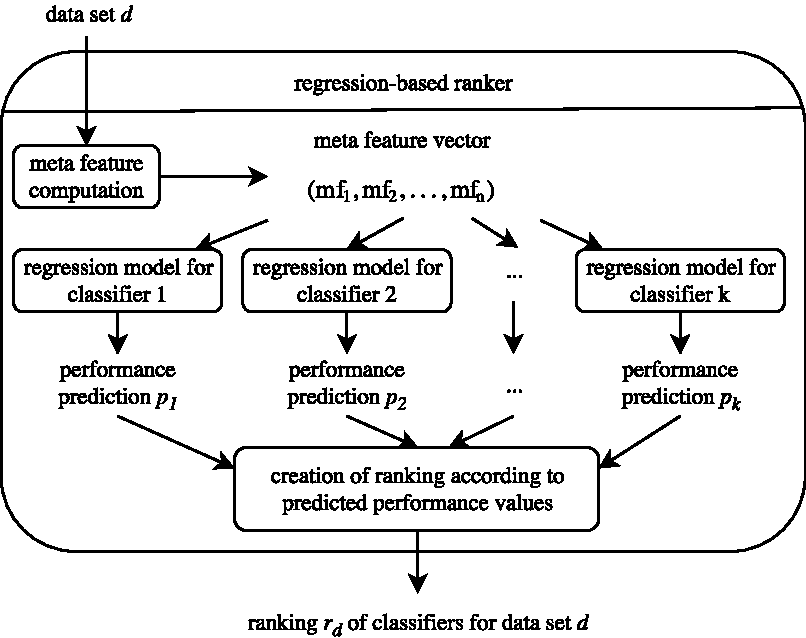
\includegraphics[scale=1]{gfx/regression_models.pdf}
\caption{An overview of how a regression-based ranker constructs a ranking.}
\label{fig:regression_ranker_model}
\end{figure}

\subsection{Preference-Based Ranking}
% How is the preference ranking done
The second possibility considered in this context is using preference learning to predict a ranking. Each instance of the data set generated beforehand (see Tab. \ref{tab:performanceValues}) contains meta feature information for the considered data set and performance values of all classifiers. The performance values can be converted to preference information by sorting the corresponding classifiers by their performance values for each data set, similar to the prediction step of the regression alternative, which is the first step of building the ranker. This leads to an ordering of classifiers associated with each instance, and implies that the preference learning task at hand is label ranking. In this case, in contrast to the regression-based approach, there exists only one model, a label ranking model. To complete the training of the ranker, this model is built with the training data that has been converted to a label ranking data set in the previous step. To make predictions, the computed meta data for a new data set is fed to this model, which consequently returns an ordering of classifiers, which is depicted in Figure \ref{fig:preference_ranker_model}. Thereby, it attempts to learn the mapping from meta features to an ordering of classifiers directly.

\begin{table}[h]
\centering
	\begin{tabularx}{\textwidth}{X | X | X | X | X}
		%\hline
		MF 1				& MF 2				& ... 	& MF n				& Ranking 	\\ \hline
		$v_{11}$			& $v_{12}$			& ...	& $v_{1n}$			& $r_1$		\\ 
		$v_{21}$			& $v_{22}$			& ...	& $v_{2n}$			& $r_2$		\\
		...				& ...				& ...	& ...				& ...		\\
		$v_{m1}$			& $v_{m2}$			& ... 	& $v_{mn}$			& $p_m$		 
	\end{tabularx}
	\label{tab:preferenceTable}
	\caption{How the preference ranker processes the training data. The ranker is trained with a table containing meta features and a ranking of classifiers for each data set.}
\end{table}

\begin{figure}
\centering
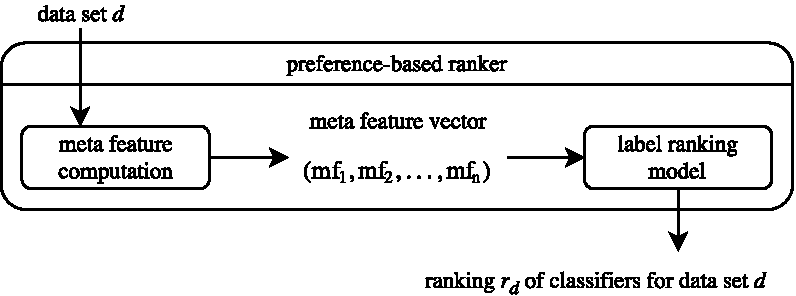
\includegraphics[scale=1]{gfx/label_ranking_model.pdf}
\caption{An overview of how a preference-based ranker constructs a ranking.}
\label{fig:preference_ranker_model}
\end{figure}

\subsection{Comparison}

While both of the ranking approaches above are used for the same purpose of ranking classification algorithms, they differ in some aspects that are interesting to point out. First, they theoretically do not require the same kind of training data. While the preference ranker only needs rankings, the regression ranker requires the exact performance data of all considered classifiers on the data sets. Although here it does not make a difference, since the performance values are computed anyways as the regression ranker utilizes them, in cases where only rankings of classifiers for a data set are known or performance values are estimated in a way that is biased, but has the same bias for all classifiers, so that the ranking is not influenced, this may be an advantage. Furthermore this leads to the curios case that training examples for the regression ranker are not directly samples from the target function the ranker learns. The target function for the regression ranker (as for the preference ranker) maps meta features of a data set to a ranking. However, for the regression ranker, the training examples have to include the actual performance values, meaning that they are of the form (\textit{meta features}, \textit{performance values}). 

Also, the approaches behave differently regarding the addition (or deletion) of a data set or classifier. If a classifier is added, for the regression-based approach, a regression model needs to be added to the ranker. Therefore, performance values for the classifier for the data set would need to be available or have to be computed anew. For the preference-based approach, however, the whole label ranking model, therefore the whole ranker, would need to be trained again, as for every data set, the ranking of classifiers has changed. Here a regression ranker conceptually has an advantage. The deletion of a classifier is much simpler: for the regression-based ranker, one regression model has to be deleted, which does not affect the other models, and in the case of the preference ranker, in the rankings produced by the label ranking model the unwanted classifier can just be removed from the rankings.

For the addition of a data set, the situation is unfavorable for both rankers. Since a new training example would be added to each regression model, they all need to be trained again on the now extended training data. For the preference ranker, likewise a new training example is added to the training data, and a new model has to be trained. The same is the case for the deletion of a data set.

Regarding training and prediction, conceptually, the preference ranker has the advantage that it both only needs to build one model and to have one model make a prediction for a new data set. On the other hand, the regression ranker needs to build as many models as there are classifiers in consideration, and also have as many models predict a performance value for their respective classifiers, which then also have to be turned into a ranking. In general, this indicates a better scalability of the preference-based approach regarding the number of classifiers (unless they are to be added dynamically) and data sets, although of course this also depends on the specific algorithms used. 

\section{Implementation}

The implementation of the rankers themselves is relatively straightforward with the theory of the previous sections in mind. However, since the goals for his thesis includes the development of an AutoML tool that returns a ranking of classification algorithms when given a data sets, the scope of the implementation goes beyond the ranking algorithms, including also pre-processing steps and means of evaluation for the rankers, relevant parts of the implementation are described in the following paragraphs; it is notable that all implementations were carried out in Java, particularly Java 8.

As mentioned before, the implementations of the ranking approaches are relatively close to the theory and will therefore not be described in detail, except for a few notable parts. First, since the tool relies on external libraries for the learning algorithms, these need to be pointed out. For the implementation of the regression models, WEKA was used, a popular libary of machine learning algorithms that includes algorithms for classification, regression, and provides help in the evaluation of these learning algorithms \cite{hall2009weka}. Regarding the preference algorithms, the jPL framework was used \cite{intelligent2017jpl}. The jPL framework is a Java framework for the evaluation of preference learning algorithms, it implements several tasks from the context of preference learning, including label ranking, and also provides a representation for data sets that contain label ranking information. 

Furthermore, so far, the descriptions of the `performance measure' used for the classifiers, that is the measure according to which the classifiers are ranked, for example the error rate or predictive accuracy, have been kept non-specific. Likewise, although the measure used in the evaluation in this thesis is predictive accuracy, the implementation has been kept general to allow any measure to be used with the rankers, as long as it is numeric.

Another fact worth mentioning regarding the implementation of the rankers is that both the regression-based approach and the preference-based approach are implemented in a way that abstract superclasses handle the data set conversions and other necessary tasks, so that it is very easy to add a new ranker implementation. For example, to create a new ranker that uses random forest as a regression model for each classifier, it is only necessary to override a method called \texttt{buildRegressionModels} which has the classifiers mapped to the training data necessary for the regression model of each classifier as a parameter and is responsible for the generation of the regression models. How this method is implemented in the case of random forest is illustrated in Figure \ref{lst:randomForest}. Here we can see that the regression model that has been acquired by training on the provided data is saved together with the classifier for which it predicts performance values. Later, this model is used to predict the performance value of that specific classifier. 

\begin{figure}
\begin{lstlisting}
@Override
protected void buildRegressionModels
			(Map  Classifier, Instances> train) 
			throws Exception {
	regressionModels = new HashMap<Classifier,Classifier>();
	for (Classifier classifier : train.keySet()) {
		RandomForest forest = new RandomForest();
		forest.buildClassifier(train.get(classifier));
		regressionModels.put(classifier, forest);
	}
}
\end{lstlisting}
\caption{A source code excerpt for a ranker based on the random forest algorithm.}
\label{lst:randomForest}
\end{figure}

Last, while the computation of the meta features is included in the workflow of a ranker in the theoretical explanations of the previous sections, meta features are calculated separately in the implementation since it is a repeating task, to speed up the evaluation of classifiers. The list of meta features used is taken from OpenML \cite{OpenML2013}, a website that not only provides a large number of openly accessible data sets, but also records performance values of learning algorithms on these data sets, and features properties of data sets. Thus the meta features were calculated with the help of an implementation provided by OpenML in its Evaluation Engine \cite{openMLEvaluationEngine}; the full list of meta features is included in Table \ref{tab:metaFeatureDetails} in the Appendix. Like the choice which classifier and performance measure to use, the choice of which meta features to be used in the implementation can be changed flexibly.

In addition to this ranking functionality, methods for the evaluation of both classifiers and rankers are implemented. Although WEKA offers capabilities for the evaluation of classifiers, additional functionality had to be added, as for example the desired estimation procedure of stratified Monte Carlo cross-validation was not supported by WEKA at the time of the implementation. Furthermore, since for the evaluation of the rankers (to build the table depicted in Tab. \ref{tab:performanceValues}), many classifiers had to be evaluated on a large number of data sets, an efficient way to execute this task was needed. This was realized by enabling the tool to take a number of jobs, consisting of classifiers and data sets, as command-line parameters, which enables execution for example on a data mining cluster. For the evaluation of rankers, the functionality needed to be built without the help of existing frameworks, and was realized in a similar way to the implemented evaluation of WEKA classifiers. It was also implemented such that after a ranker has been trained once, it can be evaluated regarding a number of different measures, to speed up the evaluation process.

Apart from the functionality described above, the implementation includes some useful recurring functions from the context of handling data sets and classifiers in the context of WEKA and OpenML. To give a general idea how the tool is structured, an overview of the package structure is given in Fig. \ref{fig:package_overview}.

\begin{figure}
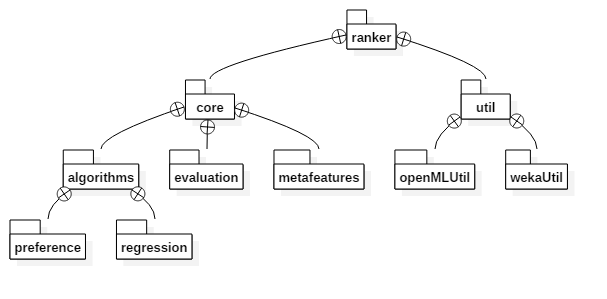
\includegraphics[width=\textwidth]{gfx/Package_Structure.png}
\caption{An overview of the package structure of the tool.}
\label{fig:package_overview}
\end{figure}
       % INCLUDE: approach
%% !TEX root = ../my-thesis.tex
%
\chapter{Implementation}
\label{sec:implementation}



 % INCLUDE: implementation
\chapter{Evaluation}
\label{sec:evaluation}

This chapter is dedicated to the evaluation of the proposed ranking approaches. First, the oracle and baseline against which the rankers are compared are explained. Second, the experimental setup, that is conditions under which the evaluation was conducted, is set forth. Last, results are presented and discussed.

\section{Baseline and Oracle}
% Workings of oracle
In order to evaluate the implemented rankers, their outputs are compared to a perfect output generated by an oracle. The oracle is implemented as a ranker that, after having been trained on a meta data - performance data set returns correct rankings when queried for any instance of that data set. The correct ranking is implied by the performance values (highest first, as the measure used here is predictive accuracy), with ties being handled in a sequential manner, i.e. for the same performance values, the algorithm that was encountered first when constructing the ranking will be ranked before all others with the same value.

% Evaluation Measures used & computed
As rankings returned by this oracle represent the ideal solution, the predicted rankings are compared with them through the measures presented in chapter \ref{sec:fundamentals}. These include the Kendall rank correlation coefficient, loss and best three loss. For all three measures, it is computed if any advantage or disadvantage one solutions has is significant, by means of the Mann-Whitney U and its P-value. The regression based rankers pose a special case: internally, they predict a performance value for each classifier, which therefore can be compared to the actual performance values to show how well they are predicted. This is done by computing the root mean square error between the predicted and actual performance values. In summary, it is desirable for the rankers to come as close as possible to the correct ranking, which is reflected by a high rank correlation and a low loss and root mean square error.

% Baseline
Furthermore, we are interested in the question as to what degree knowing about the properties of a data set influences the quality of rankings. Therefore, a ranker that is agnostic of the meta features of a query data set, that is that will always return the same ranking for any data set, is used as a baseline. More specifically, a best algorithm strategy that iteratively determines a ranking by counting the number of data sets where an algorithm is the best choice, is implemented. That means the first algorithm in the best algorithm ranking is the classifier that performs best on most data sets, the second is the best on most data sets when only rankings excluding the first algorithm are considered, and so forth. This baseline is evaluated in the same way as the preference rankers; as it does not predict performance values, the root mean square error of predicted performance values cannot bet computed. Ideally, rankings returned by the preference and regression based rankers should then be statistically significant better than the baseline. 

\section{Experimental Setup}
In the following paragraphs, it is briefly summarized under which conditions the experiments which led to the results discussed in the next section where observed. This includes which classifiers, data sets and meta features where chosen in the evaluation, what the specifications of the machines the evaluation was executed on where, how the evaluation was carried out, and which specific regression based and preference based implementations where used.

% Which classifiers 
The classifiers considered in the rankings were the learning algorithms implemented in WEKA that are fit for classification, excluding meta and ensemble methods. The full list of the 22 classifiers can be gathered from Table \ref{tab:bestAlgorithmRanking}. They where all used in their default configurations as specified by WEKA. 

% Which data sets
Data sets for the analysis where gathered from OpenML. From all data sets considered as 'active' on OpenML, which yields 2050 data sets that have been approved with no severe issues found for them so far \cite{openMLGuide}, all data sets that comply with the constraints of the learning problem at hand where selected. Only data sets with a defined, nominal target feature that are in the .ARFF format which where not specifically designed for streaming analysis\footnotemark{} where considered, which resulted in a reduced selection of 812 instances. Since this amount of data sets hindered the evaluation considerably, large data sets with more than 1000 instances or 100 features where removed as well, leading to a final selection of 448 data sets. Even though evaluation was only carried out on the shorter list, both the list of 812 and 448 data sets are included in the supplementary material for completeness.

\footnotetext{Data sets that contained the substring 'BNG' in their name for Bayesian Network Generator, which contain data artificially generated by a Bayesian Network \cite{van2014algorithm} for the sake of data stream analysis where not included in the evaluation.}

% How base performance data generated
The performance data of the classifiers for the selected data sets was generated on a linux cluster, each node consisting of two Intel(R) Xeon(R) E5-2670 processors running at 2.6GHz, 16GB RAM with usage of up to 150 nodes. There was a timeout of eight hours set for the computation of a single performance value of a classifier on a data set. For each of the classifiers, the predictive accuracy (the percentage of correctly classified instances in the data set) was recorded on each data set by means of five times stratified Monte-Carlo cross validation with a 70/30 split in training and test data. When a timeout occurred or the evaluation failed otherwise, the predictive accuracy was set to zero.

%TODO integrate DONT FORGET META FEAUTRES (WHY EVERYTHING X2??)
for mann-whitney U apache commons implementation used with ties averaged and NaNs removed before analysis
apache commons implementation for Kendall Rank correlation as well
JAICore implementation for stratified split of data set

% How rest of the evaluation carried out
All other experiments where carried out on a Windows Machine running Windows 10 Education (version 1709) with a Intel(R) Core(TM) i5-4200U CPU running at 1.60GHz (2.30GHz max) with 12 GB RAM. It is notable that especially the time-related results are to be viewed in regard to this setup. No timeouts where used in this evaluation, and the rankers where evaluated on the training data by means of leave-one-out estimation, that is for the n data sets for which performance values where recorded, they where trained with the meta data - performance examples for n - 1 data sets, and queried for the remaining data set. As n = 448 in this case, the detailed values for each data set are not included in the discussion of the results. They can, however, be found in the supplementary material, offering clues to how each ranker performed in the prediction of a ranking for each of the used data sets, identified by their ID on OpenML. 

% How find best version of preference and regression ranker
Furthermore, four alternatives where selected for a regression based and preference based alternative each, to get a general idea of how well the respective approach might be suited for the problem. For the regression based approach, the algorithms chosen where random forest, REPTree, M5P, and linear regression. For all of them, the WEKA implemenation \cite{hall2009weka} was used, and the algorithms where used with the standard hyperparameters set by WEKA. As the preference based ranking falls under the category of label ranking, and in the jPL-framework, which was used for the implementation of the label ranking algorithms and data set representations, only two alternatives for label ranking are implemented \cite{intelligent2017jpl}, the other two alternatives where generated by modifying the hyperparameters. The implemented alternatives are label ranking by pairwise comparison and instance based label ranking. As in early tests it became apparent that the instance based approach might hold more potential, for label ranking by pairwise comparison, only the default configuration dictated by jPL was used. For instance based label ranking, the default configuration, a configuration where the rank aggregation algorithm used by the label ranker was set to Kemeny-Young, and a configuration with Kemeny-Young rank aggregation and the number of neighbors of the base learner of the label ranker, namely k nearest neighbor (kNN), set to the square root of the number of instances in the training data set. In the following section, these eight variants are compared with the baseline and oracle mentioned in the previous section, and among each others.

\section{Results}

In the following subsections, results of the evaluation are discussed in detail. First, the quality of the predictions of the rankers is examined. Then, the times required for building the rankers and for predictions made as well as for the calculation of the meta features is reviewed. Last, additional insights gathered during the evaluation are pointed out.

\subsection{Accuracy}

When looking at the results depicted in Table \ref{tab:evaluationResults}, it must first be noted that positive findings regarding the Kendall rank correlation can be reported. For the full set of meta data, six out of the eight implemented alternatives outperform the baseline, all of them significantly, as can be learned from Table \ref{tab:significanceResults} which shows the results of the significance tests, with random forest having the highest correlation of 0.495. In contrast, the two approaches that did not overtake the baseline, instance based label ranking in the default configuration and label ranking by pairwise comparison, show a significant disadvantage compared to the baseline, and thus also compared to the other ranking approaches. Regarding loss, only linear regression and random forest show a significant advantage, with all label ranking approaches except for instance based label ranking having a significant disadvantage in contrast. Moving on to best three loss, the picture largely remains the same, except that surprisingly, REPTree now also has a significant advantage over the baseline. The lowest value here is achieved by random forest with a best three loss of 1.308, in comparison to 2.440 for the best algorithm baseline. These values are illustrated in Figure \ref{fig:lossGraphics}, with a scatter plot for individual best three loss values on the data sets.

Compared to the evaluation on the full set of meta data, the results on the reduced set without out probing are less distinctive. For the Kendall Rank correlation, linear regression, M5P and random forest are significantly better than the baseline, and for label ranking, both of the instance based approaches with non-default parameters as well, while the other label ranking approaches are significantly worse than the baseline. In total, random forest is still the best alternative with a correlation of 0.439, slightly worse than the correlation achieved on the full meta data. For both loss measures however, while the disadvantages of the label ranking approaches remain, none of the eight alternatives achieves a significantly better loss or best three loss than the baseline anymore.

Summarizing the observed results, in general, a regression based approach shows an indication to be stronger than a preference based approach. Specifically, using random forest as a regression model is the best solution observed in the evaluation, and label ranking by pairwise comparison the weakest, as it falls behind the other ranking approaches and the baseline often.

\begin{landscape}
\begin{table}[h]
\centering
	\resizebox{23,7cm}{!}{%
	\begin{tabularx}{27cm}{>{\hsize=2.8\hsize}X | >{\hsize=.8\hsize\raggedleft\arraybackslash}X | >{\hsize=.8\hsize\raggedleft\arraybackslash}X | >{\hsize=1\hsize\raggedleft\arraybackslash}X  >{\hsize=.8\hsize\raggedleft\arraybackslash}X | >{\hsize=.8\hsize\raggedleft\arraybackslash}X | >{\hsize=.8\hsize\raggedleft\arraybackslash}X | >{\hsize=1\hsize\raggedleft\arraybackslash}X  >{\hsize=.8\hsize\raggedleft\arraybackslash}X| >{\hsize=.8\hsize\raggedleft\arraybackslash}X | >{\hsize=.8\hsize\raggedleft\arraybackslash}X | >{\hsize=1\hsize\raggedleft\arraybackslash}X  >{\hsize=.8\hsize\raggedleft\arraybackslash}X}
		Ranker 				& \multicolumn{4}{>{\hsize=4.0\hsize\centering\arraybackslash}X}{Kendall's Rank Correlation} & \multicolumn{4}{>{\hsize=4.0\hsize\centering\arraybackslash}X}{Loss} & \multicolumn{4}{>{\hsize=4.0\hsize\centering\arraybackslash}X}{BestThreeLoss}\\ \cline{2-13}
							 			& Min	& Max	& Mean			  & $\pm$Stdv  & Min & Max  & Mean			 & $\pm$Stdv   & Min	& Max	 & Mean			  & 	$\pm$Stdv  \\ \hline
		LinearRegression 				& -0.255 & 0.896 & $\bullet$ 0.473 & $\pm$0.221 & 0 & 86.667 & $\bullet$ 3.469 & $\pm$7.244  & 0 & 31.220  & $\bullet$ \textbf{1.267} & $\pm$3.011 \\
		M5P				 				& -0.290 & 0.870 & $\bullet$ 0.470 & $\pm$0.219 & 0 & 82.353 & 3.780	 		 & $\pm$6.535  & 0 & 82.353  & $\bullet$ 1.508 & $\pm$4.757 \\	
		RandomForest		 				& -0.281 & 0.922 & $\bullet$ \textbf{0.495} & $\pm$0.228 & 0 & 60.000 & $\bullet$ \textbf{3.097} & $\pm$5.745  & 0 & 34.634  & $\bullet$ 1.308 & $\pm$3.150 \\	
		REPTree			 				& -0.229 & 0.896 & $\bullet$ 0.412 & $\pm$0.213 & 0 & 82.353 & 4.829	 		 & $\pm$7.948  & 0 & 34.634  & 1.759	 		  & $\pm$3.515 \\	
		InstanceBased 					& -0.429 & 0.870 & $\circ$ 0.221	  & $\pm$0.249 & 0 & 82.353 & $\circ$ 5.401 	 & $\pm$9.440  & 0 & 82.353  & $\circ$ 3.620	  & $\pm$8.540 \\	
		InstanceBased\footnotemark{}		& -0.429 & 0.887 & $\bullet$ 0.340 & $\pm$0.252 & 0 & 98.367 & 5.437 			 & $\pm$10.323 & 0 & 82.353  & 3.294	 		  & $\pm$8.367 \\	
		InstanceBased\footnotemark{}		& -0.429 & 0.870 & $\bullet$ 0.335 & $\pm$0.249 & 0 & 82.353 & $\circ$ 5.382	 & $\pm$9.402  & 0 & 82.353  & $\circ$ 3.511	  & $\pm$8.493 \\	
		PairwiseComparison 				& -0.870 & 0.576	 & $\circ$ 0.014	  & $\pm$0.234 & 0 & 97.822 & $\circ$ 9.762	 & $\pm$13.135 & 0 & 82.353  & $\circ$ 4.001	  & $\pm$8.600 \\	
		BestAlgorithm	 				& -0.351 & 0.758 & 0.296	 		  & $\pm$0.213 & 0 & 82.353 & 4.480 			 & $\pm$9.205  & 0 & 82.353  & 2.440 		  & $\pm$7.625 \\							\hline \hline
		\addtocounter{footnote}{-2}
		LinearRegression 				& -0.532 & 0.835 & $\bullet$ 0.350 & $\pm$0.235 & 0 & 82.353 & 4.921	 		 & $\pm$9.109  & 0 & 82.353 & 2.211	 		& $\pm$6.744 \\
		M5P				 				& -0.290	 & 0.887 & $\bullet$ 0.344 & $\pm$0.219 & 0 & 87.455 & 5.367	 		 & $\pm$9.662  & 0 & 82.353 & 2.060	 		& $\pm$5.466 \\	
		RandomForest		 				& -0.359 & 0.913 & $\bullet$ \textbf{0.439} & $\pm$0.233 & 0 & 82.353 & \textbf{3.538} & $\pm$6.803  & 0 & 40.000 & \textbf{1.587} & $\pm$3.784 \\	
		REPTree			 				& -0.290 & 0.844 & 0.301			  & $\pm$0.215 & 0 & 91.154 & $\circ$ 6.771	 & $\pm$10.710 & 0 & 82.353 & $\circ$ 3.013	& $\pm$7.162 \\	
		InstanceBased 					& -0.429 & 0.870 & $\circ$ 0.221	  & $\pm$0.249 & 0 & 82.353 & $\circ$ 5.401 	 & $\pm$9.429  & 0 & 82.353 & $\circ$ 3.615	& $\pm$8.531 \\	
		InstanceBased\footnotemark{}		& -0.429 & 0.887 & $\bullet$ 0.340 & $\pm$0.252 & 0 & 98.367 & 5.437 			 & $\pm$10.311 & 0 & 82.353 & 3.294	 		& $\pm$8.357 \\	
		InstanceBased\footnotemark{}		& -0.429 & 0.870 & $\bullet$ 0.335 & $\pm$0.249 & 0 & 82.353 & $\circ$ 5.382	 & $\pm$9.391  & 0 & 82.353 & $\circ$ 3.511	& $\pm$8.483 \\	
		PairwiseComparison 				& -0.870 & 0.524	 & $\circ$ 0.013	  & $\pm$0.232 & 0 & 91.667 & $\circ$ 9.486	 & $\pm$13.158 & 0 & 82.353 & $\circ$ 4.096	& $\pm$8.669 \\	
		BestAlgorithm	 				& -0.351 & 0.758 & 0.296	 		  & $\pm$0.213 & 0 & 82.353 & 4.479 			 & $\pm$9.205  & 0 & 82.353 & 2.440 			& $\pm$7.625 \\						
	\end{tabularx}
	}
	\caption{Evaluation results with full meta data (top) and no probing (bottom). The \textbf{best mean}, $\bullet$ significant advantages, and $\circ$ significant disadvantages are marked as  such.}
	\label{tab:evaluationResults}
\end{table}

\addtocounter{footnote}{-2}
\stepcounter{footnote}\footnotetext{Rankaggregation: Kemeny-Young}
\stepcounter{footnote}\footnotetext{Rankaggregation: Kemeny-Young, Baselearner KNN with k=$\sqrt{\text{number of instances}}$}
\end{landscape}

\begin{table}[h]
\resizebox{\textwidth}{!}{%
\hspace{-1cm}
	\begin{tabularx}{\textwidth}{>{\hsize=1.3\hsize}X | >{\hsize=0.9\hsize\raggedleft\arraybackslash}X | >{\hsize=0.9\hsize\raggedleft\arraybackslash}X | >{\hsize=0.9\hsize\raggedleft\arraybackslash}X}
		Ranker 						& \multicolumn{3}{>{\hsize=3.0\hsize\centering\arraybackslash}X}{P-Value}\\ \cline{2-4} 
									& \multicolumn{1}{>{\centering\arraybackslash}X}{Kendall's Rank Correlation} & \multicolumn{1}{>{\centering\arraybackslash}X}{Loss} & \multicolumn{1}{>{\centering\arraybackslash}X}{B3L} \\ \hline
		LinearRegression 			& 5.798E-30 		& 0.030 		& 0.001 \\
		M5P				 			& 1.831E-29 		& 0.888		& 0.012 \\
		RandomForest		 			& 1.208E-35 		& 0.006 		& 0.001 \\
		REPTree			 			& 4.471E-14 		& 0.076 		& 0.607 \\
		InstanceBased				& 6.540E-6 		& 0.012 		& 0.002 \\
		InstanceBased\footnotemark{}	& 0.012			& 0.089 		& 0.077 \\
		InstanceBased\footnotemark{}	& 0.014 			& 0.038 		& 0.012 \\
		PairwiseComparison			& 5.457E-59 		& 1.702E-22 	& 1.451E-9 \\ 
		\hline \hline \addtocounter{footnote}{-2}
		LinearRegression 			& 2.955E-4		& 0.118		& 0.568 \\
		M5P				 			& 0.007			& 0.070		& 0.929 \\
		RandomForest		 			& 1.278E-18		& 0.118		& 0.067 \\
		REPTree			 			& 0.808			& 1.781E-7 	& 0.004 \\
		InstanceBased				& 6.540E-6 		& 0.012		& 0.002 \\
		InstanceBased\footnotemark{} & 0.012 		& 0.089		& 0.077 \\
		InstanceBased\footnotemark{} & 0.014			& 0.038		& 0.012 \\
		PairwiseComparison			& 1.310E-59		& 2.016E-22	& 2.587E-10 \\
	\end{tabularx}
	}
	\caption{Significance of evaluation results (compared to the baseline) with full meta data (top) and no probing (bottom).}
	\label{tab:significanceResults}
\end{table}


\addtocounter{footnote}{-2}
\stepcounter{footnote}\footnotetext{Rankaggregation: Kemeny-Young}
\stepcounter{footnote}\footnotetext{Rankaggregation: Kemeny-Young, base learner KNN with k=$\sqrt{\text{number of instances}}$}

\tikzsetnextfilename{LossGraphics}
\begin{figure}
%\pgfplotsset{width=\textwidth}
\resizebox{\textwidth}{!}{%
\begin{tikzpicture}
\begin{axis}[
	title=regular scale,
	height=\textwidth,
	width=\textwidth,
	ylabel={BestThreeLoss}, 
	xlabel={Data Set},
]
\addplot [mark=*,only marks,mark size=1pt] table [x=ID,y=BestThreeLoss,col sep=semicolon] {data/BestAlgorithmRanker_metaData_small_allPerformanceValues.csv};
\addplot [mark=*,only marks,mark size=1pt,uniaccentblue] table [x=ID,y=BestThreeLoss,col sep=semicolon] {data/RandomForestRanker_metaData_small_allPerformanceValues.csv};
\addplot [very thick,mark=none,black,samples=2,domain=0:450]{2.440};
\addplot [very thick,mark=none,uniaccentblue,samples=2,domain=0:450]{1.308};
\addplot [very thick,mark=none,uniaccentblue,samples=2,domain=0:450]{0};
\legend{BestAlgorithm, RandomForest, BestAlgorithm (mean), RandomForest (mean)}
\end{axis}
\end{tikzpicture}%
~%
%
\begin{tikzpicture}
\begin{axis}[
	title=log scale (base 2),
	height=\textwidth,
	width=\textwidth,
	ylabel={BestThreeLoss}, 
	xlabel={Data Set},
	ymode=log,
	log basis y={2}
]
\addplot [mark=*,only marks,mark size=1pt] table [x=ID,y=BestThreeLoss,col sep=semicolon] {data/BestAlgorithmRanker_metaData_small_allPerformanceValues.csv};
\addplot [mark=*,only marks,mark size=1pt,uniaccentblue] table [x=ID,y=BestThreeLoss,col sep=semicolon] {data/RandomForestRanker_metaData_small_allPerformanceValues.csv};
\addplot [very thick,mark=none,black,samples=2,domain=0:450]{2.440};
\addplot [very thick,mark=none,uniaccentblue,samples=2,domain=0:450]{1.308};
\addplot [very thick,mark=none,uniaccentblue,samples=2,domain=0:450]{0};
\legend{BestAlgorithm, RandomForest, BestAlgorithm (mean), RandomForest (mean)}
\end{axis}
\end{tikzpicture}
}
\caption{The best three loss for the baseline compared to the random forest ranker (full meta data).}
\label{fig:lossGraphics}
\end{figure}


\subsection{Computation Times}

Because the ranking itself is implemented as a means of speeding up the process of algorithm selection, the time it takes to rank is not negligible. The full results of how long it takes to build the respective ranking models and how much time they need for predictions can be taken from Table \ref{tab:times}. Results are rounded to the full millisecond, as due to the times being measured with a stop watch in the code, more accurate measurements are not possible. The times for building the regression rankers are not surprising; the regression models take far more time to be built than most of the label ranking methods, most likely due to the fact the regression based rankers have to train 22 regression models in order to be trained themselves. However, it is notable that while the ranking by Pairwise Comparison was not among the best solutions concerning the accuracy of the results, it is the ranker with the highest mean build time for full meta data, and second highest for a reduced meta data set, whereas in other cases the high quality of results is correlated with a high time invested in the building of the ranker. The Random Forest ranker, for example, is the ranker with the highest build time, and also with the rankings of the generally highest quality. But the most important fact to be taken away from Table \ref{tab:times} is that the prediction times for all rankers are short enough to be negligible, with the mean prediction time never being higher than five milliseconds and the maximum never exceeding 50 milliseconds. Furthermore, while the build times are higher, these are not as important due to the fact that each model only needs to be trained once. Although in a real-world scenario, calculation times for meta features also have to be taken into account when ranking, which therefore will be discussed in the following paragraph.

\begin{table}[h]
	\begin{tabularx}{1.1\textwidth}{>{\hsize=2.6\hsize}X | >{\hsize=.8\hsize}X | >{\hsize=.8\hsize}X | >{\hsize=.8\hsize}X | >{\hsize=.8\hsize}X| >{\hsize=.8\hsize}X | >{\hsize=.8\hsize}X | >{\hsize=.8\hsize}X | >{\hsize=.8\hsize}X}
		Ranker 				& \multicolumn{4}{>{\hsize=4.0\hsize\centering\arraybackslash}X}{Ranker Build Time (ms)} & \multicolumn{4}{>{\hsize=4.0\hsize\centering\arraybackslash}X}{Ranker Prediction Time (ms)} \\ \cline{2-9}
										& Min		& Max		& Mean		& Stdv 	& Min	& Max		& Mean		& Stdv 	\\ \hline
		LinearRegression 				& 1454 		& 2060 		& 1580	 	& 36 	& 0 		& 1      	& 0	 	    & 0 	\\
		M5P				 				& 3145 		& 4916 		& 3226	 	& 89 	& 0 		& 16		 	& 0	 		& 1	\\	
		RandomForest		 				& 6048 		& 9720 		& 6236	 	& 259 	& 0		& 16 		& 3	 		& 2	\\	
		REPTree			 				& 599 		& 1264 		& 629		& 38 	& 0 		& 16			& 1	 		& 16	\\	
		InstanceBased 					& 66 		& 550 		& 90	 		& 25 	& 0 		& 47			& 5 			& 8	\\	
		InstanceBased\footnotemark{}		& 66 		& 138 		& 88	 		& 12 	& 0 		& 19		 	& 1			& 3	\\	
		InstanceBased\footnotemark{}		& 66 		& 163		& 87	 		& 12 	& 0 		& 16		 	& 1		 	& 2	\\	
		PairwiseComparison 				& 8456 		& 15063 		& 9096	 	& 449 	& 0 		& 16 		& 0	 		& 2	\\	
		BestAlgorithm	 				& 204	 	& 1250		& 227	 	& 52	 	& 0		& 0			&  0 		& 0\\	
		\hline \hline
		LinearRegression 				& 421 		& 500 		& 446	 	& 10 	& 0 		& 0      	& 0	 	    & 0 	\\
		M5P				 				& 2219 		& 4225 		& 2282	 	& 148 	& 0 		& 16		 	& 0	 		& 1	\\	
		RandomForest		 				& 6175 		& 10535 		& 5419	 	& 479 	& 0		& 16 		& 3	 		& 6	\\	
		REPTree			 				& 484 		& 1078 		& 509		& 32 	& 0 		& 15			& 0	 		& 1	\\	
		InstanceBased 					& 62 		& 141 		& 77	 		& 7  	& 0 		& 16			& 4 			& 7	\\	
		InstanceBased\footnotemark{}		& 62 		& 125 		& 79	 		& 8 		& 0 		& 16		 	& 1			& 3	\\	
		InstanceBased\footnotemark{}		& 62 		& 110		& 77	 		& 7  	& 0 		& 16		 	& 1		 	& §	\\	
		PairwiseComparison 				& 6705 		& 7893		& 7253	 	& 169 	& 0 		& 16 		& 0		 	& 2	\\	
		BestAlgorithm	 				& 206	 	& 405		& 232	 	& 23	 	& 0		& 0			&  0 		& 0\\				
	\end{tabularx}
	\label{tab:times}
	\caption{Build and Prediction Times of the Rankers Rounded to Full Milliseconds with Full Meta Features (Top) and Without Probing (Bottom)}
\end{table}


\addtocounter{footnote}{-2}
\stepcounter{footnote}\footnotetext{Rankaggregation: Kemeny-Young}
\stepcounter{footnote}\footnotetext{Rankaggregation: Kemeny-Young, Baselearner KNN with n=$\sqrt{\text{number of instances}}$}

Table \ref{tab:metaFeatureTimes} shows the times required for the computation of groups of meta features as discussed in chapter \ref{sec:approach}. As can be taken from the table, the computation of the full meta features takes approximately 135 milliseconds on average, while the simple meta features without probing add approximately 3 milliseconds to the prediction times on average. Regarding these computation times it is also notable that among the probing meta feature groups, some are considerably more expensive than others, so that in the future it might be sensible to consider only light probing with probing meta feature groups that are not as expensive.

\begin{table}[h]
	\begin{tabularx}{\textwidth}{>{\hsize=3.0\hsize}X | >{\hsize=.5\hsize}X | >{\hsize=.5\hsize}X | >{\hsize=.5\hsize}X | >{\hsize=.5\hsize}X}
		Meta Feature Group & \multicolumn{4}{>{\hsize=2.0\hsize\centering\arraybackslash}X}{Computation Time (ms)}\\ \cline{2-5}
									& Min		& Max		& Mean		& Stdv\\ \hline			
	NominalAttDistinctValues 		& 0			& 16		& 0.127		& 1.128\\
	SimpleMetaFeatures				& 0 		& 16		& 0.221		& 1.614\\
	Cardinality						& 0			& 19		& 0.654		& 2.723\\
	Statistical						& 0			& 69		& 1.520		& 5.442\\
	DecisionStump, 2 folds			& 0 		& 54		& 1.536		& 4.710\\
	RandomTreeDepth1, 2 folds		& 0			& 29		& 1.955		& 4.785\\
	RandomTreeDepth2, 2 folds		& 0			& 18		& 2.114		& 4.793\\
	RandomTreeDepth3, 2 folds 		& 0			& 30		& 1.636		& 4.454\\
	REPTreeDepth1, 2 folds			& 0			& 56		& 2.980		& 6.805\\
	REPTreeDepth2, 2 folds			& 0			& 67		& 2.955		& 6.999\\
	REPTreeDepth3, 2 folds			& 0			& 60		& 3.259		& 7.206\\
	J48.001., 2 folds				& 0			& 201		& 5.129		& 13.935\\ 
	J48.0001., 2 folds				& 0			& 101		& 4.944		& 10.657\\
	J48.00001., 2 folds				& 0 		& 116		& 4.464		& 10.744\\
	NaiveBayes, 2 folds				& 0			& 200		& 6.853		& 17.679 \\
	kNN1N, 2 folds					& 0			& 1118		& 22.250	& 69.212\\
	CfsSubsetEval kNN1N, 2 folds	& 2			& 1096		& 25.806	& 52.236\\
	CfsSubsetEval NaiveBayes, 2 folds &	2		& 132		& 23.304	& 12.918\\
	CfsSubsetEval DecisionStump, 2 folds & 2	& 150		& 23.087	& 12.296\\			
	\end{tabularx}
	\caption{Computation Times for Groups of Meta Features}
	\label{tab:metaFeatureTimes}
\end{table}


\subsection{Further Insights}

Further insights to be noted are the accuracy of predictions of performance values for classifiers by the regression models, and the static ranking constructed by the best algorithm baseline. The accuracy of the predictions achieved by the regression based rankers are depicted in Table \ref{tab:rootMeanSquareError}, for full and reduced meta data respectively. The first thing that attracts attention in this table is the absurdly high values for Linear Regression and M5P, however, these are all caused by the very high maximum value on one data set with id 685. If these extreme maxima remain out of consideration for Linear Regression and M5P (the other algorithms do not have this problem) more reasonable values are obtained. For M5P, on the full meta data the new maximum is 311.526, mean 8.127 and standard deviation 18.407; on the reduced meta data it is a maximum of 474.692, mean 15.444 and standard deviation 27.433. For Linear Regression, on the full meta data the new maximum is 142.996, mean 9.281 and standard deviation 8.438; on the reduced meta data it is a maximum of 131.456, mean 14.351 and standard deviation 10.299. However, these values are still worse than the ones obtained for the Random Forest and REPTree variants. It comes as little surprise that the Random Forest Ranker also delivers the most accurate results for performance estimates, but as these best values are more than 6\% off on average for the full meta data and even more than 10\% off on average for the reduced meta data, it is questionable whether these prediction can be useful. The usefulness is dependent on the task these predictions would be used for an whether if requires very accurate predictions of performance values.

\begin{table}[h]
	\begin{tabularx}{\textwidth}{>{\hsize=1.8\hsize}X | >{\hsize=.8\hsize}X | >{\hsize=.8\hsize}X | >{\hsize=.8\hsize}X | >{\hsize=.8\hsize}X}
		Ranker 				& \multicolumn{4}{>{\hsize=4.0\hsize\centering\arraybackslash}X}{Root Mean Square Error} \\ \cline{2-5}
										& Min		& Max		& Mean		& Stdv 	\\ \hline
		LinearRegression 				& 1454 		& 2060 		& 1580	 	& 36 	\\
		M5P				 				& 3145 		& 4916 		& 3226	 	& 89 	\\	
		RandomForest		 			& 6048 		& 9720 		& 6236	 	& 259 	\\	
		REPTree			 				& 599 		& 1264 		& 629		& 38 	\\	\hline \hline
		LinearRegression 				& 1454 		& 2060 		& 1580	 	& 36 	\\
		M5P				 				& 3145 		& 4916 		& 3226	 	& 89 	\\	
		RandomForest		 			& 6048 		& 9720 		& 6236	 	& 259 	\\	
		REPTree			 				& 599 		& 1264 		& 629		& 38 	\\							
	\end{tabularx}
	\label{tab:rootMeanSquareError}
	\caption{Root Mean Square Error of Predicted Performance Values for the Regression-Based Rankers (full meta data)}
\end{table}

The second interesting thing to consider is the ranking which is created by the best algorithm baseline. This ranking constitutes meta-knowledge about the learning process itself in that it shows which algorithms are generally a good choice for many data sets. This ranking is depicted in Table \ref{tab:bestAlgorithmRanking}. The table is to be read top to bottom; of the 22 algorithms, the algorithm in the ith row is placed first on most data sets when compared to the next 22-i algorithms. The associated number represents the number of data sets on which the algorithm was placed first. It is, however, not a particularly surprising result, as for example the placement of Random Forest as the first algorithm was to be expected. Random Forest is a learning algorithm that is known to often deliver good performances, which was proven again in the results discussed previously - out of the reviewed ranking approaches, Random Forest was the best choice.

\begin{table}[h]
\centering
	\begin{tabularx}{\textwidth}{X | X}
		%\hline
		Classifier				&	Number of Data Sets Placed First \\	\hline
		RandomForest				&	80								\\	\hline
		MultilayerPerceptron		&	66								\\	\hline
		BayesNet					&	51								\\	\hline
		Naive Bayes				&	448								\\	\hline	
		Logistic					&	50								\\	\hline	
		SGD						&	65								\\	\hline
		SMO						&	313								\\	\hline
		SimpleLogistic			&	131								\\	\hline
		LMT						&	120								\\	\hline	
		IBk						&	66								\\	\hline	
		KStar					&	95								\\	\hline	
		DecisionTable			&	88								\\	\hline
		JRip						&	117								\\	\hline
		PART						&	104								\\	\hline
		J48						&	140								\\	\hline	
		REPTree					&	110								\\	\hline
		RandomTree				&	133								\\	\hline	
		OneR						&	177								\\	\hline						
		DecisionStump			&	253								\\	\hline
		VotedPerceptron			&	255								\\	\hline	
		ZeroR					&	378								\\	\hline	
		NaiveBayesMultinomial	&	6								\\	\hline	
	\end{tabularx}
	\label{tab:bestAglorithmRanking}
	\caption{The Ranking of Classifiers returned by the Best Algorithm Baseline}
\end{table}








     % INCLUDE: evaluation
\chapter{Related Work}
\label{sec:related}
% Of course much work in this field and cannot possibly cover all of this so confined to closely related or well-known / state of the art
The demand for aid in the process of selecting an algorithm has already led to the development of numerous solutions that automate machine-learning (AutoML). In the following sections, the workings of a few such tools that are related to this work are outlined briefly, loosely organized by their scope of operation. Each tool's usage of meta knowledge is discussed shortly.\\ 

\section{Predicting Rankings}
%% Ranking
% Incorporating times
In contrast to ranking solely based on classifier performances, \citeauthor{DBLP:journals/ml/AbdulrahmanBRV18} investigated an approach to extend existing ranking methods by incorporating the time needed for the evaluation of the classifier \cite{DBLP:journals/ml/AbdulrahmanBRV18}. They call this combined measure of accuracy and time A3R, and integrate it into to different ranking approaches.

% Rank aggregation A3R
One of those two approaches is called average-ranking. It utilizes meta knowledge to suggest a ranking of classifiers for a new data sets, which in this case consist of recorded past performances of classifiers on data sets. That means this algorithms aggregates the performances of classifiers on all rankings once and then always recommends the same ranking. The new measures is integrated here by, instead of ordering only according to performance values, the classifiers are ordered according to the combined measure A3R.

% Active testing A3R


% Introduce loss curves and how the measure influences them


\section{Algorithm and Hyperparameter Selection}
%% CASH
Taking it a step further than predicting rankings of classification algorithms with fixed hyperparameters are tools that in addition two selecting an algorithm also optimize its hyperparameters, which has been defined as 'the combined algorithm selection and hyperparameter optimization problem (short: CASH)' \cite{thornton2013auto}. Two widely used approaches of this kind are AUTO-WEKA and AUTO-SKLEARN. It has to be noted that thus these approaches also go further than the solution proposed in this thesis, which currently only takes into account one fixed hyperparameter configuration for each classification algorithm. 

% Auto-WEKA
Auto-WEKA is an AutoML tool that both selects a machine learning algorithm and optimizes its hyperparameters by using Bayesian optimization \cite{thornton2013auto}. It was first released in 2013 as an extension to the popular data mining software WEKA \cite{hall2009weka}, which also offers a user-friendly GUI in addition to a command-line interface and an API, to assist the large number of novice users of the software in selecting parameterized algorithms for their problems. The tool has since grown in popularity and is in version 2.0 as of March 2016 \cite{kotthoff2016auto}. In Auto-WEKA, the problem of selecting an algorithm and its hyperparameters is combined by treating the algorithm itself as a hyperparameter and searching the joint space of algorithms and hyperparameters for the best solution. An input data set is first preprocessed by means of feature selection. Then, Sequential Model-Based Optimization for General Algorithm Configuration (SMAC) is used to 'iterate[...] between fitting models and using them to make choices about which configurations to investigate' \cite{hutter2011sequential}. In the case of Auto-WEKA, this means that during the optimization process, a model is built, a configuration of hyperparameters that is promising regarding the current model and training data is tried out, and the result is fed back to the model. This cycle is then repeated until the allocated time has run out. Auto-WEKA exploits meta-knowledge, that is considering past performances of algorithms, to make decisions by always trying algorithms like Random Forest, which perform well on a large number of data sets, first. \\

% SK-learn
AUTO-SKLEARN has been described as a sister-package to Auto-WEKA and is an AutoML tool which is based on scikit-learn, a machine learning library for Python \cite{feurer2015efficient}. It works very similar to AutoML but extends it by adding a meta-learning pre-processing step to warmstart the Bayesian optimization and automatically constructing ensembles during optimization. During the pre-processing phase, performance values for the classifiers available in AUTO-SKLEARN are recorded on a set of data sets. For each data set, the algorithm which shows the best empirical performance is noted. Then, certain meta-features are calculated for each data set. The first step of the tool when given a new problem is to calculate meta-features of the data set. Then, the Manhattan distance to the other data sets is determined according to the meta-features, and the algorithms that are associated with the k-nearest data sets are used as a starting point for further optimization. The authors observe that the additional meta-learning and ensemble construction result in a more efficient and robust application. Their results show that meta-learning can be used to improve the overall AutoML process.\\

\section{Constructing pipelines}
%% Whole pipelines
Before a classifier is evaluated on a data set, often a number of pre-processing steps are executed first. These could include selecting promising features and discarding other and normalizing the data. The 'sequence of tasks that need to be performed to classify instances belonging to a given dataset into a set of predefined categories' \cite{DBLP:conf/eurogp/SaPOP17} can therefore be defined as a machine learning pipeline. Two tools which construct such complete pipelines for data sets are MP-Plan and the RECIPE framework.

% ML-Plan
ML-Plan is an AutoML tool that instead of concentrating on hyperparameter optimization, aims to optimize the whole machine-learning pipeline \cite{wever2017automatic}. This is achieved by viewing machine-learning as a task, building a hierarchical task network out of those tasks, and then searching for a solution in the induced tree structure. In the tree, the root node contains the complex task of building a machine learning pipeline, inner nodes represent incomplete pipelines consisting of complex and possibly also primitive tasks, and leaf nodes are complete pipelines that include only primitive tasks. An example of this might be 'classify' as the root node, with an intermediate node on some level that contains the tasks 'build NN', 'train NN' and 'predict from NN'. The complex task 'build NN' would then further be decomposed, and could lead to a leaf node with n tasks 'Add layer', 'build NN' and 'predict from NN', which are all primitive tasks that do not need to be further decomposed. A best-first search algorithm in a modified variant is then used to find good solutions in this task network. For the actual implementation of the learning algorithms, WEKA is used. While this variant does not use meta-learning in the process of optimizing the pipeline, the authors find that their results exceed those achieved by Auto-WEKA.\\

\tikzsetnextfilename{MLPlanTasks}
\begin{figure}
\tikzset{edge from parent/.style={draw,->}}
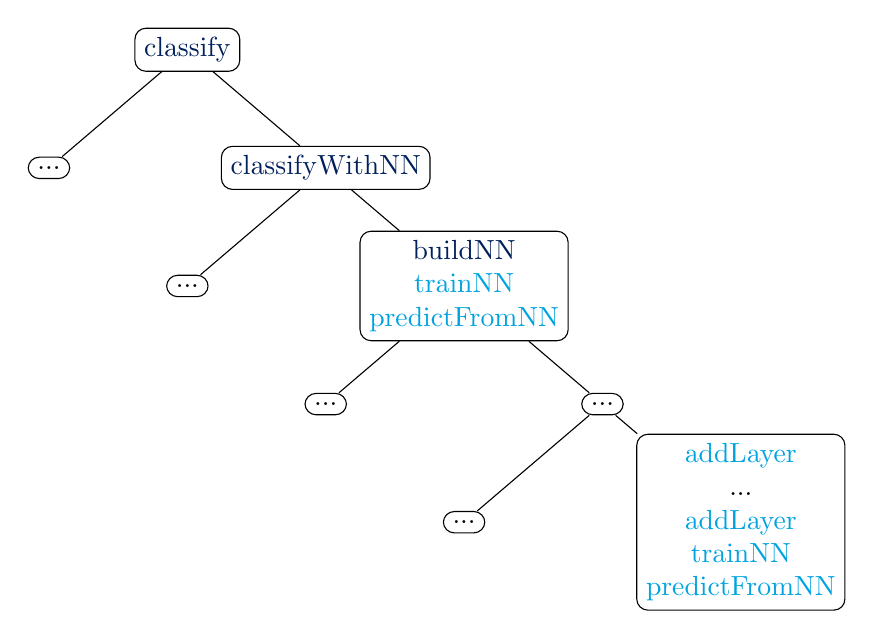
\begin{tikzpicture}[sibling distance=10em,
  every node/.style = {shape=rectangle, rounded corners,
    draw, align=center}]]
  \node {\textcolor{uniblue}{classify}}
    child { node {...} }
    child { node {\textcolor{uniblue}{classifyWithNN}}
    child { node {...} }
      child { node {\textcolor{uniblue}{buildNN} \\ \textcolor{uniaccentblue}{trainNN} \\ \textcolor{uniaccentblue}{predictFromNN}}
        child { node {...} }
        child { node {...} 
          child { node {...}  }
          child { node {\textcolor{uniaccentblue}{addLayer} \\ ... \\ \textcolor{uniaccentblue}{addLayer} \\ \textcolor{uniaccentblue}{trainNN} \\ \textcolor{uniaccentblue}{predictFromNN} } } } }
    };
\end{tikzpicture}
\caption{An example for how the complex task 'classify' might be broken down by ML-Plan. The figure is loosely adapted from \cite{wever2017automatic}. Nodes containing '...' represent an undefined number of subtrees. \textcolor{uniblue}{Complex tasks} and \textcolor{uniaccentblue}{primitive tasks} are distinguished by their color.}
\label{fig:mltree}
\end{figure}

% Recipe framework
Similar to ML-PLAN, the RECIPE framework constructs whole classification pipelines for new problems \cite{DBLP:conf/eurogp/SaPOP17}. However, this is done by means of grammar-based genetic programming: the tasks that the pipeline is composed of are represented by a grammar, which 'is used to generate the initial population, as well as to constraint the crossover and mutation operations, which always need to be valid according to the grammar' \cite{DBLP:conf/eurogp/SaPOP17}. This means that generated individuals representing complete pipelines can never be invalid. So for a new data set combined with a grammar that represents the valid pipelines, the tool first initializes the first generation according to the grammar. The fitness of individuals is then evaluated by mapping them to their respective implementations in the scikit-learn framework, and a new generation is created that takes this newly gained information into account. Evaluation by the authors indicates that the RECIPE framework is able to compete with AUTO-SKLEARN and a different evolutionary approach, although it does not incorporate meta-knowledge in the search.   % INCLUDE: related work
% Move from specific to general
% Use existing literature for confirmation, contradiction, comparison
% "Speak to introduction"
\chapter{Conclusion}
\label{sec:conclusion}
% Introductory restatement of research problems, aims / reseach question -> remin of problem + purpose and how addressed
In this thesis, the problem of predicting a ranking of classification algorithms for a new data set on the basis of meta features of the data set and past performances of the algorithms has been considered. Being able to predict a ranking of such algorithms is desirable since this potentially speeds up and simplifies the process of algorithm selection, which is important due to a rapidly increasing amount of available data, and more importantly, data that is available but has not yet been analyzed. The problem has been addressed by implementing to different approaches, regression-based and preference-based ranking, and the evaluations of both against each other, a baseline and an oracle.

% Summary of findings and limitations: what has been covered
- Results - 

% Practical applications / limitations: assess value / relevance / implications: What does it mean for theory, what for practice
On the basis of the results, it can be concluded that a causal connection exists between certain meta features of a data set and the predictive accuracy of classification algorithms for this data set, which can be exploited to a degree by regression models and label ranking models to predict a ranking of classification algorithms. A practical application of these findings may be to incorporate the implementation or parts of it in another Auto-ML tool as a search heuristic, similar to how some Auto-ML solutions like AUTO-SKLEARN already benefits from meta learning \cite{feurer2015efficient}. However, some additional work may have to be done in extension to this thesis in order for a sensible integration.

% Recommendations for future work
\section{Future Work}
\label{sec:conclusion:future}
% Has worked reasonably well -> extend evaluation


%- more careful training by hand-selecting datasets for training (but then aains is this really the real world anymore? But then again duplicates may be contained)




- use this to try to predict other measures (e.g. time needed)
- look at the loss curve + loss-time (log) curve
- further investigate the better solution
- integrate solution into other auto ml solution if sensible regarding time contraints for that solution (and accuracy)
-e.g. use A3R
- or runtime could be predicted separately by nn based on meta data \cite{DBLP:journals/corr/abs-1709-07615}
- adding feature pre-processing

% Extension of the tool
- better fitting of learning algorithms to meta data (more manual work, but of course consider danger of overfitting!

% Extended evaluation
- compare against other tools that rank r.g. the Jan van Rijn one
- deeper analysis of meta features, e.g. add some, remove some, consider trade-off time accuracy

% Use this for predicting different algorithms
So far, the evaluation of the tool has been confined to predicting algorithms for classification. Since this has been relatively successful, it could be tested whether similar predictions can also be made for other machine learning tasks like regression or clustering. 

- hyperparameters neglected here, may include standard combinations in future work (or random ones)-> possible only if id by string
- use this for regression

an average baseline like used in speeding up algo select might be better     % INCLUDE: conclusion

% --------------------------
% Back matter
% --------------------------
\appendix\cleardoublepage
% !TEX root = ../my-thesis.tex
%
\chapter{Appendix}
\label{sec:appendix}


\section{Appendix Section 1}
\label{sec:appendix:sec1}

\begin{table}[h]
	\begin{tabularx}{\textwidth}{X | X | X}
		%\hline
		Alpha		& Beta			& Gamma			\\ \hline
		0			& 1				& 2				\\ \hline
		3			& 4				& 5				\\ %\hline
	\end{tabularx}
	\label{tab:table1}
	\caption{This is a caption text.}
\end{table}
       % INCLUDE: appendix
%
{%
\setstretch{1.1}
\renewcommand{\bibfont}{\normalfont\small}
\setlength{\biblabelsep}{0pt}
\setlength{\bibitemsep}{0.5\baselineskip plus 0.5\baselineskip}
\printbibliography[nottype=online]
\printbibliography[heading=subbibliography,title={Webpages},type=online,prefixnumbers={@}]
}
\cleardoublepage

\listoffigures
\cleardoublepage

\listoftables
\cleardoublepage

% !TEX root = ../my-thesis.tex
%
\pagestyle{empty}
\hfill
\vfill
\pdfbookmark[0]{Colophon}{Colophon}
\section*{Colophon}

This thesis was typeset with \LaTeXe.
It uses the \textit{Clean Thesis} style developed by Ricardo Langner.
The design of the \textit{Clean Thesis} style is inspired by user guide documents from Apple Inc.

Download the \textit{Clean Thesis} style at \url{http://cleanthesis.der-ric.de/}.

\cleardoublepage

% !TEX root = ../my-thesis.tex
%
%************************************************
% Declaration
%************************************************
\pdfbookmark[0]{Declaration}{Declaration}
\chapter*{Declaration}
\label{sec:declaration}
\thispagestyle{empty}

You can put your declaration here, to declare that you have completed your work solely and only with the help of the references you mentioned.

\bigskip

\noindent\textit{\thesisUniversityCity, \thesisDate}

\smallskip

\begin{flushright}
	\begin{minipage}{5cm}
		\rule{\textwidth}{1pt}
		\centering\thesisName
	\end{minipage}
\end{flushright}

%*****************************************
%*****************************************

\clearpage
\newpage
\mbox{}

% **************************************************
% End of Document CONTENT
% **************************************************
\end{document}
